\documentclass[a4paper,12pt]{article}

\usepackage[utf8]{inputenc}
\usepackage[T1]{fontenc}
\usepackage[brazil]{babel}
\usepackage{graphicx}
\usepackage{booktabs}
\usepackage{geometry}
\usepackage{float}

\geometry{margin=2.5cm}

\title{Grafos -- Implementação N3}
\author{Mateus Vasconcellos}
\date{Maio 2026}

\begin{document}

\maketitle

\section{Introdução}

Este trabalho apresenta os resultados obtidos na implementação do algoritmo de caminho mínimo utilizando uma versão modificada do algoritmo de Dijkstra. Foram realizados testes em diferentes tipos de grafos, analisando o desempenho em relação ao número de vértices, distância mínima encontrada, quantidade de arestas do caminho e tempo de execução.

% ----------------------------------------------------
% Resultados
% ----------------------------------------------------

\section{Resultados}

\subsection{Grafo Aleatório Esparso}

\begin{table}[H]
\centering
\caption{Tabela 1 -- Grafo Aleatório Esparso}
\begin{tabular}{lrrrr}
\toprule
Instância & Vértices & Distância mínima & Arestas & Tempo (ms) \\
\midrule
tipo1\_pequeno & 50 & 32 & 3 & 0 \\
tipo1\_medio & 500 & 103 & 7 & 1 \\
tipo1\_grande & 5000 & 298 & 7 & 8 \\
tipo1\_enorme & 50000 & 968 & 6 & 53 \\
\bottomrule
\end{tabular}
\end{table}

\subsection{Grafo em Grade (Grid)}

\begin{table}[H]
\centering
\caption{Tabela 2 -- Grafo em Grade (Grid)}
\begin{tabular}{lrrrr}
\toprule
Instância & Vértices & Distância mínima & Arestas & Tempo (ms) \\
\midrule
tipo2\_pequeno & 100 & 165 & 18 & 0 \\
tipo2\_medio & 900 & 980 & 58 & 0 \\
tipo2\_grande & 10000 & 5011 & 198 & 2 \\
tipo2\_enorme & 90000 & 28791 & 598 & 36 \\
\bottomrule
\end{tabular}
\end{table}

\begin{figure}[H]
\centering
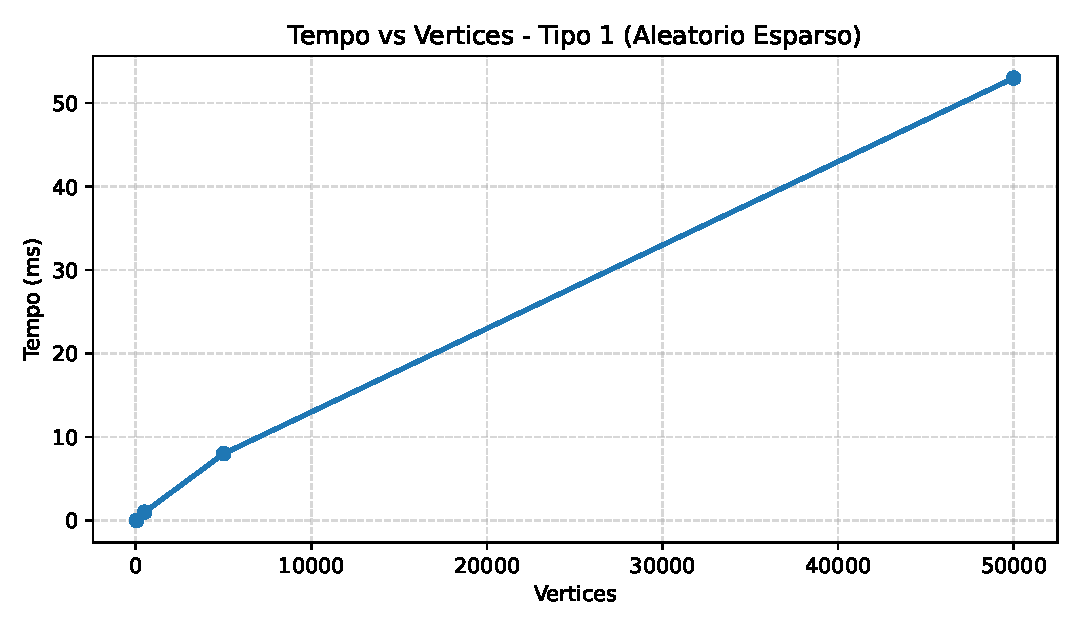
\includegraphics[width=0.85\linewidth]{grafico_tempo_tipo1.pdf}
\caption{Figura 1 -- Tempo vs Vértices (Tipo 1 -- Aleatório Esparso)}
\end{figure}

\begin{figure}[H]
\centering
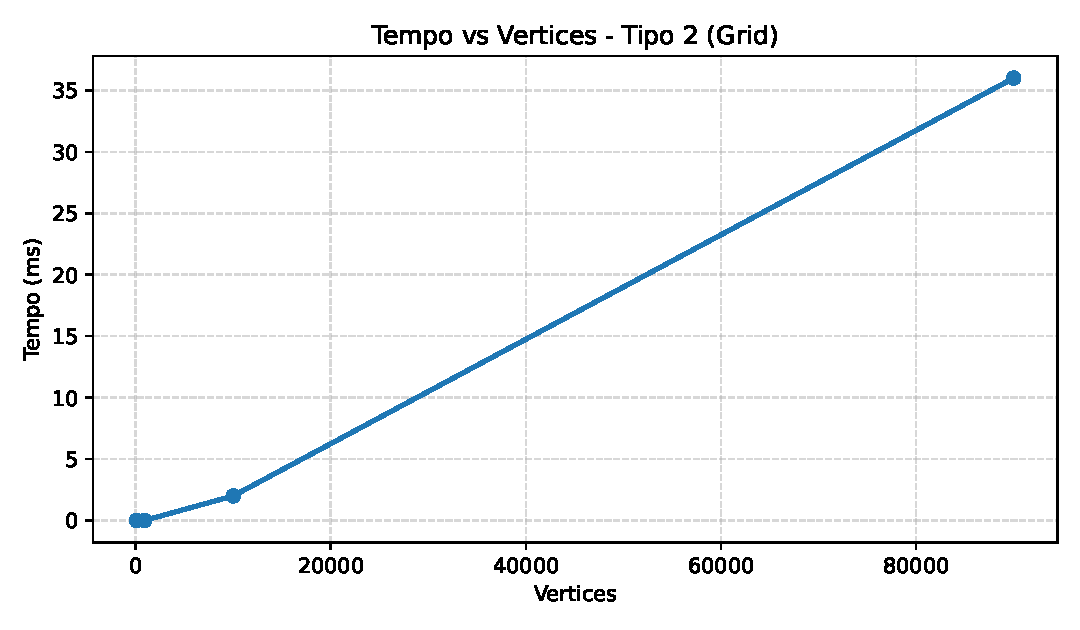
\includegraphics[width=0.85\linewidth]{grafico_tempo_tipo2.pdf}
\caption{Figura 2 -- Tempo vs Vértices (Tipo 2 -- Grid)}
\end{figure}

% ----------------------------------------------------
% Saídas de exemplo
% ----------------------------------------------------

\section{Saídas de Exemplo}

\subsection{Tipo 1 (Pequeno)}

\begin{verbatim}
=======================================================
  Caminho Minimo - grafos/tipo1_pequeno.txt
=======================================================
  Origem  : 0
  Destino : 49
-------------------------------------------------------
  Comprimento (peso)   : 32
  Numero de arestas    : 3
  Vertices do caminho  : 0 -> 44 -> 48 -> 49
=======================================================
\end{verbatim}

\subsection{Tipo 2 (Pequeno)}

\begin{verbatim}
=======================================================
  Caminho Minimo - grafos/tipo2_pequeno.txt
=======================================================
  Origem  : 0
  Destino : 99
-------------------------------------------------------
  Comprimento (peso)   : 165
  Numero de arestas    : 18
  Vertices do caminho  : 
  0 -> 1 -> 11 -> 21 -> 22 -> 32 -> 42 -> 43 -> 44
  -> 54 -> 64 -> 65 -> 66 -> 67 -> 77 -> 87
  -> 88 -> 89 -> 99
=======================================================
\end{verbatim}
